% Тут используется класс, установленный на сервере Papeeria. На случай, если
% текст понадобится редактировать где-то в другом месте, рядом лежит файл matmex-diploma-custom.cls
% который в момент своего создания был идентичен классу, установленному на сервере.
% Для того, чтобы им воспользоваться, замените matmex-diploma на matmex-diploma-custom
% Если вы работаете исключительно в Papeeria то мы настоятельно рекомендуем пользоваться
% классом matmex-diploma, поскольку он будет автоматически обновляться по мере внесения корректив
%
\documentclass{matmex-diploma}
\usepackage{algpseudocode}
\usepackage{algorithm}
\usepackage{caption}
\usepackage{algorithmicx}
\usepackage{amssymb}

\begin{document}

\algtext*{EndWhile}% Remove "end while" text
\algtext*{EndIf}% Remove "end if" text
\algtext*{EndFor}% Remove "end for" text
\algtext*{EndFunction}% Remove "end function" text

% Год, город, название университета и факультета предопределены,
% но можно и поменять.
% Если англоязычная титульная страница не нужна, то ее можно просто удалить.
\filltitle{ru}{
    chair              = {Кафедра системного программирования},
    title              = {Синтаксический анализ регулярных множеств},
    type               = {diploma},
    position           = {студентка},
    group              = 544,
    author             = {Вербицкая Екатерина Андреевна},
    supervisorPosition = {ст. пр., магистр информационных технологий},
    supervisor         = {Григорьев С.\,B.},
    reviewerPosition   = {программист ООО "ИнтеллиДжей Лабс", \\магистр прикладной математики и информатики},
    reviewer           = {Бреслав А.\,А.},
    chairHeadPosition  = {д.\,ф.-м.\,н., профессор},
    chairHead          = {Терехов А.\,Н.},
    city               = {Санкт-Петербург},
    year               = {2015}
}
\filltitle{en}{
    chair              = {Chair of Software Engineering},
    title              = {Parsing of Regular Sets},
    author             = {Ekaterina Verbitskaia},
    supervisorPosition = {Senior Lecturer},
    supervisor         = {Semen Grigorev},
    reviewerPosition   = {Software Developer at IntelliJ Labs},
    reviewer           = {Andrey Breslav},
    chairHeadPosition  = {Professor},
    chairHead          = {Andrey Terekhov},
}
\maketitle
\tableofcontents

\section*{Введение}

Ручное управление памятью в языках, подобных C++, является источником большого количества трудно отслеживаемых ошибок, наличия которых можно было бы
избежать, сделав процесс управления памятью автоматическим. \textit{Сборка мусора} является одним из способов автоматического управления памятью, при
котором освобождение памяти выводится из-под контроля ПО на прикладном уровне. При автоматическом управлении программист не может явно влиять на распределение
объектов в памяти, у него есть лишь
косвенные способы сделать это с помощью использования тех или иных языковых конструкций. В идеальном случае, для рационального использования
памяти необходимо освобождать память, занимаемую объектами, которые более не будут использованы программой. Поскольку точно определить, что
объект не будет использован в дальнейшем, невозможно, на практике используют критерий доступности. \textit{Доступность} --- это консервативное
приближение используемости. \textit{Мусором}, в таком случае, называют объект, все пути доступа к которому уже разрушены, а память из-под него
ещё не освобождена. В некоторое, заранее определенное время, например, в простейшем случае, когда перестаёт хватать свободной памяти, выполнение
программы временно приостанавливается и запускается процесс \textit{сборки мусора}, который освобождает всю или ту, что возможно, память,
занятую мусором, после чего управление возвращается обратно программе. \textit{Сборщиком мусора} называется компонент, производящий \textit{сборку мусора}.

Процесс \textit{сборки мусора}, в простейшем случае, делят на три этапа:
\begin{enumerate}
\item \textit{Построение корневого множества}. На этом этапе строится множество объектов, которые считаются изначально доступными.
Такие объекты называются \textit{корнями} (англ. roots). Данное построение
аксиоматично, т.е. основывается на некотором наборе правил, согласно которым те или иные элементы считаются доступными. Данный этап является неотъемлемой
частью любого сборщика мусора.
\item \textit{Маркировка}. Начиная с множества, построенного на предыдущем этапе, происходит сканирование памяти, и все объекты, до которых возможно
добраться из построенного корневого множества, считаются доступными; оставшиеся объекты считаются мусором.
\item \textit{Освобождение}. Происходит сканирование кучи, в течение которого память из-под всех элементов, помеченных как мусор или не отмеченных как
доступные, освобождается.
\end{enumerate}

Есть несколько требований, которые должны быть выполнены для реализации сборки мусора:
\begin{enumerate}
\item Возможность построения корневого множества. Иными словами, необходимо иметь возможность идентифицировать все указатели в программном стеке, регистрах
и статической области памяти.
\item Должна присутствовать возможность определить все указатели из любого объекта на другие элементы кучи.
\end{enumerate}
В таких языках, как LISP или JAVA все условия соблюдаются, и в них успешно используется технология сборки мусора, в то время как, например,
в языке C не все условия выполняются. В языках, где не соблюдаются хотя бы одно из вышеперечисленных условий, возможна исключительна
\textit{консервативная сборка мусора}.
\textit{Консервативной} называется такая сборка мусора, при которой любой элемент данных, значение которого может быть истолковано, как указатель на
некоторый элемент кучи, считается  таковым. Консервативный подход к сборке мусора не позволяет собрать весь мусор, что может стать проблемой при обработке
большого количества данных. Неконсервативная сборка мусора лишена подобного недостатка и способна освободить всю память программы, более не
являющуюся доступной. \textit{Неконсервативным} или  \textit{точным сборком мусора} называется сборщик мусора, имеющий возможность точно распознать
все указатели в памяти. Иными словами, точный сборщик мусора --- это сборщик мусора, не использующий консервативный подход.

В C++ не соблюдаются требования, необходимые для сборки сборки мусора, реализовать точный сборщик мусора без ограничений
на использование некоторых примитивов языка не представляется возможным.
Более того, в C++ имеется ряд технических сложностей, затрудняющих реализацию точного сборщика мусора.
Тем не менее, в случае соблюдения программистом некоторых соглашений на програмный код,
точная сборка мусора становится возможной и в C++.

Целями работы является реализация основных примитивов библиотеки неконсервативной сборки мусора для C++,
обеспечение возможности совмещения ручного и автоматического управления памятью.
\section{Постановка задачи}
Целью данной работы является разработка алгоритма ослабленного синтаксического 
анализа для регулярной аппроксимации множества значений динамически формируемого
выражения, который для всех корректных относительно некоторой эталонной 
грамматики цепочек строит конечное представление множества деревьев разбора, при
этом цепочки, не принадлежащие эталонному языку, игнорируются.

В рамках данной дипломной работы поставлены следующие задачи.
\begin{itemize}
  \item Разработать алгоритм синтаксического анализа динамически формируемых 
        выражений, поддерживающий работу с произвольными входными графами.
  \item Реализовать предложенный алгоритм.
  \item Доказать корректность алгоритма.
  \item Провести апробацию.
\end{itemize}
\section{Обзор}
Предлагаемый в данной работе алгоритм заимствует распространённые принципы существующих работ данной области. Помимо этого переиспользуется RNGLR-алгоритм синтаксического анализа вместе с соответствующими структурами данных. В данном разделе приведён обзор подходов к анализу встроенных языков, дано краткое описание RNGLR-алгоритма, а также описан проект, в рамках которого велась разработка предложенного алгоритма.

\subsection{Подходы к анализу динамически формируемых выражений}
Анализ встроенных языков начинается с поиска и выделения в исходном коде основной программы так называемых \emph{точек интереса} или \emph{хотспотов} (hotspot), в которых осуществляется исполнение или передача формируемого выражения выделенной компоненте. Определение точек интереса обычно производится либо с помощью пользователя, посредством аннотаций или явного указания соответствующих строк исходного кода, либо автоматически, если есть некоторые знания об используемом фреймворке. Например, на хотспот могут указывать такие функции как \textsc{exec} динамического SQL. В точке интереса производится вычисление множества значений динамически формируемого выражения, а также его последующая аппроксимация. Следующим шагом, как правило, производится токенизация, то есть по языку над алфавитом символов строится язык над алфавитом терминалов эталонной грамматики. Затем полученный язык может анализироваться (синтаксически и семантически) в зависимости от стоящей задачи. Перечисленные шаги не обязательно производятся последовательно, более того, некоторые из них могут быть опущены. 

Под \emph{регулярной аппроксимацией} мы подразумеваем аппроксимирование множества значений динамически формируемого выражения некоторым регулярным выражением. В терминах, привычных для задач распознавания, проверка корректности выражений из аппроксимирующего множества формулируется как задача проверки включения регулярного языка в эталонный, как правило, контекстно-свободный, язык, которая разрешима во многих важных на практике случаях~\cite{LangInclusion}. Многие существующие работы по анализу встроенных языков используют такой подход. В работе~\cite{Stranger} для построения аппроксимации используется анализ прямой достижимости (forward reachability analysis), дальнейший анализ основан на распознавании образцов (pattern detection) в аппроксимирующем множестве или генерации некоторого конечного подмножества строк для анализа с помощью отдельных инструментов. В работе~\cite{JSA} построение регулярной аппроксимации осуществляется посредством расширения контекстно-свободной аппроксимации, построенной во время анализа исходного кода основной программы. Предложенный нами подход вдохновлён проектом Alvor~\cite{Alvor,Alvor2}, который использует технику, основанную на GLR-алгоритме, для синтаксического анализа регулярной аппроксимации. В данном проекте для упрощения задачи синтаксического анализа, регулярный язык над алфавитом символов сначала трансформируется в регулярный язык над алфавитом терминалов эталонной грамматики с помощью специальной процедуры лексического анализа. 

В серии работ~\cite{AbstrParsing,LRAbstrParsing,LRAbstrParsingSema} предложен подход, основанный на явном представлении множества формируемых выражений в виде системы уравнений потока данных (data-flow equations). В качестве базы алгоритма синтаксического анализа выбран традиционный LALR(1)-алгоритм, при этом переиспользуются таблицы управления. Синтаксический анализ производится во время решения уравнений потока данных в домене абстрактных стеков. Проблема возможного бесконечного роста стеков, возникающая в общем случае, разрешается с помощью абстрактной интерпретации (abstract interpretation~\cite{AbstractInterpretation}). Впоследствии данный подход был расширен вычислением семантики с помощью атрибутных грамматик, что позволило анализировать более широкий, чем LALR(1), класс грамматик. 

\subsection{RNGLR-алгоритм}
RNGLR-алгоритм (Right-Nulled Generalized LR) является модификацией предложенного Масару Томитой алгоритма Generalized LR (GLR)~\cite{Tomita}, предназначенного для анализа естественных языков. GLR-алгоритм был предназначен для анализа неоднозначных контекстно-свободных грамматик. Неоднозначности грамматики порождают конфликты сдвиг/свёртка (shift/reduce) и свёртка/свёртка (reduce/reduce). GLR-алгоритм использует управляющие таблицы, схожие с управляющими таблицами LR-алгоритма, ячейки которых могут содержать несколько действий. Основная идея GLR-алгоритма состоит в проведении всех возможных действий во время синтаксического анализа. При этом для эффективного представления множества стеков и деревьев вывода используются особые структуры данных, основанные на графах.

Оригинальный алгоритм, предложенный Томитой, не был способен анализировать все контекстно-свободные грамматики. Элизабет Скотт и Адриан Джонстоун предложили RNGLR-алгоритм, который расширяет GLR-алгоритм специальным способом обработки обнуляемых справа правил (right-nullable rules, имеющих вид $\mathrm{A} \rightarrow \alpha \beta$, где $\beta$ выводит пустую строку $\epsilon$).

\begin{algorithm}[!ht]
\begin{algorithmic}[1]
\caption{RNGLR-алгоритм}
\label{rnglr}
\Function{parse}{$grammar, input$}
  \State{$\mathcal{R} \gets \emptyset$} \Comment{Очередь троек: вершина GSS, нетерминал,\par
       \hskip2.5cm длина свёртки}
  \State{$\mathcal{Q} \gets \emptyset$} \Comment{Коллекция пар: вершина GSS, состояние парсера}
  \If{$input = \epsilon$}
    \If{$grammar$ accepts empty input} {report success}
    \Else { report failure}
    \EndIf
  \Else
    \State{\Call{addVertex}{$0, 0, startState$}}
    \ForAll{$i$ in $0..input.Length-1$}
      \State{\Call{reduce}{$i$}}
      \State{\Call{push}{$i$}}
    \EndFor
    \If{$i=input.Length-1$ and there is a vertex in the last\par 
      \hskip1cm level of GSS which state is accepting}
      \State{report success}
    \Else { report failure}
    \EndIf
  \EndIf
\EndFunction
\Function{reduce}{$i$}
  \While{$\mathcal{R}$ is not empty}
    \State{$(v, N, l) \gets \mathcal{R}.Dequeue()$}
    \State{find the set $\mathcal{X}$ of vertices reachable from $v$ along the path}
    \State{of length $(l-1)$ or length $0$ if $l=0$}
    \ForAll{$v_{h} = (level_{h}, state_{h})$ in $\mathcal{X}$}
      \State{$state_{t} \gets$ calculate new state by $state_{h}$}
      \State{    and nonterminal $N$}
      \State{\Call{addEdge}{$i, v_{h}, v.level, state_{tail}, (l=0)$}}
    \EndFor
  \EndWhile
\EndFunction
\Function{push}{$i$}
  \State{$\mathcal{Q^{'}} \gets$ copy $\mathcal{Q}$}
  \While{$\mathcal{Q^{'}}$ is not empty}
    \State{$(v, state) \gets \mathcal{Q}.Dequeue()$}
    \State{\Call{addEdge}{$i, v, v.level + 1, state, false$}}
  \EndWhile
\EndFunction
\end{algorithmic}
\end{algorithm}

\begin{algorithm}[!ht]
\begin{algorithmic}[1]
\caption{Построение GSS}
\label{RNGLRMain}
\Function{addVertex}{$i, level, state$}
  \If{GSS does not contain vertex $v = (level, state)$}
    \State{add new vertex $v = (level, state)$ to GSS}
    \State{calculate the set of shifts by $v$ and the $input[i+1]$ and}
    \State{add them to $\mathcal{Q}$}
    \State{calculate the set of zero-reductions by $v$ and the $input[i+1]$} 
    \State{and add them to $\mathcal{R}$}
  \EndIf
  \State{\Return{$v$}}
\EndFunction
\Function{addEdge}{$i, v_{h}, level_{t}, state_{t}, isZeroReduction$}
  \State{$v_{t} \gets$ \Call{addVertex}{$i, level_{t}, state_{t}$}}
  \If{GSS does not contain edge from $v_{t}$ to $v_{h}$}
    \State{add new edge from $v_{t}$ to $v_{h}$ to GSS}
    \If{not $isZeroReduction$}
      \State{calculate the set of reductions by $v$ and the $input[i+1]$}
      \State{and add them to $\mathcal{R}$}
    \EndIf
  \EndIf
\EndFunction
\end{algorithmic}
\end{algorithm}

Для эффективного представления множества стеков во время синтаксического анализа в алгоритме RNGLR используется структурированный в виде графа стек (Graph Structured Stack, GSS), который является ориентированным графом, чьи вершины соответствуют  элементам отдельных стеков, а ребра связывают последовательные элементы. Каждая вершина может иметь несколько входящих рёбер, что соответствует слиянию нескольких стеков, за счёт чего производится переиспользование общих участков отдельных стеков. Вершина GSS~--- это пара $(s,l)$, где $s$~--- состояние парсера, а $l$~--- уровень (позиция во входном потоке).

RNGLR-алгоритм последовательно считывает символы входного потока слева направо, по одному за раз, и строит GSS по ``слоям'': сначала осуществляются все возможные свёртки для данного символа, после чего сдвигается следующий символ со входа. Свёртка или сдвиг модифицируют GSS следующим образом. Предположим, что необходимо добавить ребро $(v_t,v_h)$ в GSS. По построению, конечная вершина добавляемой дуги к такому моменту уже обязательно находится в GSS. Если начальная вершина также содержится в GSS, то в граф добавляется новое ребро (если оно ранее не было добавлено), иначе создаются и добавляются в граф и начальная вершина, и ребро. Каждый раз, когда создаётся новая вершина $v=(s,l)$, алгоритм вычисляет новое состояние парсера $s'$ по $s$ и следующему символу входного потока. Пара $(v,s')$, называемая push, добавляется в глобальную коллекцию $\mathcal{Q}$. Также при добавлении новой вершины в GSS вычисляется множество $\epsilon$-свёрток, после чего элементы этого множества добавляются в глобальную очередь $\mathcal{R}$. Свёртки длины $l>0$ вычисляются и добавляются в $\mathcal{R}$ каждый раз, когда создаётся новое (не-$\epsilon$) ребро. Подробное описание работы со структурированным в виде графа стеком GSS содержится в алгоритме~\ref{RNGLRMain}.

В силу неоднозначности грамматики входная строка может иметь несколько деревьев вывода, как правило, содержащих множество идентичных поддреревьев. Для того, чтобы компактно хранить множество деревьев вывода, создано компактное представление леса разбора (Shared Packed Parse Forest, SPPF)~\cite{SPPF}. SPPF является ориентированным графом и обладает следующей структурой.
\begin{enumerate}
  \item \emph{Корень} (то есть, вершина, не имеющая входящих дуг) соответствует стартовому нетерминалу грамматики.
  \item \emph{Терминальные} вершины, не имеющие исходящих дуг, соответствуют либо терминалам грамматики, либо деревьям вывода пустой строки $\epsilon$.
  \item \emph{Нетерминальные} вершины являются корнем дерева вывода некоторого нетерминала грамматики; только вершины-продукции могут быть непосредственно достижимы из таких вершин.
  \item \emph{Вершины-продукции}, представляющие правую часть правила грамматики для соответствующего нетерминала. Вершины, непосредственно достижимые из них, упорядочены и могут являться либо терминальными, либо нетерминальными вершинами. Количество таких вершин лежит в промежутке $[l-k..l]$, где $l$~--- это длина правой части продукции, а $k$~--- количество финальных символов, выводящих $\epsilon$ (правые обнуляемые символы игнорируются для уменьшения потребления памяти).
\end{enumerate}

SPPF создаётся одновременно с построением GSS. Каждое ребро GSS ассоциировано с либо с терминальным, либо с нетерминальным узлом. Когда добавление ребра в GSS происходит во время операции push, новая терминальная вершина создаётся и ассоциируется с ребром. Нетерминальные вершины ассоциируются с ребрами, добавленными во время операции reduce. Если ребро уже было в GSS, к ассоциированной с ним нетерминальной вершине добавляется новая вершина-продукция. Подграфы, ассоциированные с рёбрами пути, вдоль которого осуществлялась свёртка, добавляются как дети к вершине-продукции. После того, как входной поток прочитан до конца, производится поиск всех вершин, имеющих принимающее состояние анализатора, после чего подграфы, ассоциированные с исходящими из таких вершин рёбрами, объединяются в один граф. Из полученного графа удаляются все недостижимые из корня вершины, что в итоге оставляет только корректные деревья разбора для входной строки. 

Алгоритм~\ref{rnglr} представляет более детальное описание алгоритма.

\subsection{Проект YaccConstructor и платформа для анализа встроенных языков}
В рамках проекта YaccConstructor~\cite{YC} лаборатории языков инструментов JetBrains на математико-механическом факультете СПбГУ проводятся исследования в области лексического и синтаксического анализа, а также статического анализа встроенных языков. Проект YaccConstructor представляет собой модульный инструмент, имеет собственный язык спецификации грамматик, объединяет различные алгоритмы лексического и синтаксического анализа. В рамках проекта была создана платформа для статического анализа встроенного кода~\cite{SECR14}; диаграмма последовательности, иллюстрирующая взаимодействие модулей платформы представлена на рис.~\ref{seq}. Цветом выделена компонента, осуществляющая синтаксический анализ множества значений динамически формируемого выражения. 
\begin{figure}[!h]
 \centering
 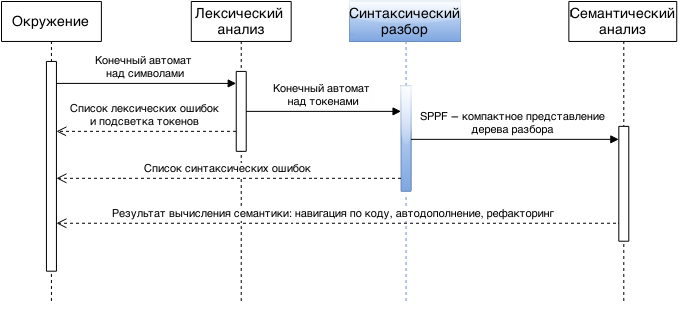
\includegraphics[width=10cm]{Verbitskaya/pics/Seq_rus.png}
 \caption{Диаграмма последовательности: взаимодействие компонентов
инструмента YaccConstructor}
 \label{seq}
\end{figure}

Предыдущая реализация платформы работала с грубой аппроксимацией, которая не осуществляла поддержку формирования выражения в циклах и с помощью строковых выражений~\cite{SECR13}. Используемая аппроксимация не являлась аппроксимацией сверху, что сказывалось на точности результатов анализа, и поэтому впоследствии она была заменена на регулярную. Однако это повлекло необходимость изменения алгоритма синтаксического анализа, чему и посвящена данная работа. 

\section{An algorithm for CFPQ using relational query semantics}
In this section, we show how the context-free path query evaluation using the relational query semantics can be reduced to the calculation of matrix transitive closure $a^{cf}$, prove the correctness of this reduction, introduce an algorithm for computing the transitive closure $a^{cf}$, and provide a step-by-step demonstration of this algorithm on a small example.

\subsection{Reducing CFPQ to transitive closure} \label{section_reducing}
In this section, we show how the context-free relations $R_A$ can be calculated by computing the matrix transitive closure $a^{cf}$.

We introduce another definition of the transitive closure of an arbitrary square matrix $a$ as $$a^{cf} = a^{(1)} \cup a^{(2)} \cup \cdots$$ where $a^{(1)} = a$ and $a^{(i)} = a^{(i-1)} \cup (a^{(i-1)} \times a^{(i-1)}), ~i \ge 2.$

To show that Valiant's and this definitions of the matrix transitive closure are equivalent, we introduce the partial order $\succeq$ on matrices with the fixed size which have subsets of $N$ as elements. For square matrices $a, b$ of the same size, we denote $a \succeq b$ iff $a_{i,j} \supseteq b_{i,j}$, for every $i, j$. For these two definitions of transitive closure, the following lemmas and theorem hold.

\begin{lemma}\label{lemma:cf_geq_valiant}
	Let $G =(N,\Sigma,P)$ be a grammar, let $a$ be a square matrix. Then $a^{(k)} \succeq a^{(k)}_+$ for any $k \geq 1$.
\end{lemma}
\begin{proof}(Proof by Induction)
	
	\textbf{Basis}: The statement of the lemma holds for $k = 1$, since $$a^{(1)} = a^{(1)}_+ = a.$$
	
	\textbf{Inductive step}: Assume that the statement of the lemma holds for any $k \leq (p - 1)$ and show that it also holds for $k = p$ where $p \geq 2$. For any $i \geq 2$ $$a^{(i)} = a^{(i-1)} \cup (a^{(i-1)} \times a^{(i-1)}) \Rightarrow a^{(i)} \succeq a^{(i-1)}.$$ Hence, by the inductive hypothesis, for any $i \leq (p-1)$ $$a^{(p-1)} \succeq a^{(i)} \succeq a^{(i)}_+.$$ Let $1 \leq j \leq (p - 1)$. The following holds $$(a^{(p-1)} \times a^{(p-1)}) \succeq (a^{(j)}_+ \times a^{(p-j)}_+),$$ since $a^{(p-1)} \succeq a^{(j)}_+$ and $a^{(p-1)} \succeq a^{(p-j)}_+$. By the definition, $$a^{(p)}_+ = \bigcup^{p-1}_{j=1}{a^{(j)}_+ \times a^{(p-j)}_+}$$ and from this it follows that $$(a^{(p-1)} \times a^{(p-1)}) \succeq a^{(p)}_+.$$ By the definition, $$a^{(p)} = a^{(p-1)} \cup (a^{(p-1)} \times a^{(p-1)}) \Rightarrow a^{(p)} \succeq (a^{(p-1)} \times a^{(p-1)}) \succeq a^{(p)}_+$$ and this completes the proof of the lemma.
\end{proof}

\begin{lemma}\label{lemma:valiant_geq_cf}
	Let $G =(N,\Sigma,P)$ be a grammar, let $a$ be a square matrix. Then for any $k \geq 1$ there is $j \geq 1$, such that $(\bigcup^{j}_{i=1}{a^{(i)}_+}) \succeq a^{(k)}$.
\end{lemma}
\begin{proof}(Proof by Induction)
	
	\textbf{Basis}: For $k = 1$ there is $j = 1$, such that $$a^{(1)}_+ = a^{(1)} = a.$$ Thus, the statement of the lemma holds for $k = 1$.
	
	\textbf{Inductive step}: Assume that the statement of the lemma holds for any $k \leq (p - 1)$ and show that it also holds for $k = p$ where $p \geq 2$. By the inductive hypothesis, there is $j \geq 1$, such that $$(\bigcup^{j}_{i=1}{a^{(i)}_+}) \succeq a^{(p-1)}.$$ By the definition, $$a^{(2j)}_+ = \bigcup^{2j-1}_{i=1}{a^{(i)}_+ \times a^{(2j-i)}_+}$$ and from this it follows that $$(\bigcup^{2j}_{i=1}{a^{(i)}_+}) \succeq (\bigcup^{j}_{i=1}{a^{(i)}_+}) \times (\bigcup^{j}_{i=1}{a^{(i)}_+}) \succeq (a^{(p-1)} \times a^{(p-1)}).$$ The following holds $$(\bigcup^{2j}_{i=1}{a^{(i)}_+}) \succeq a^{(p)} = a^{(p-1)} \cup (a^{(p-1)} \times a^{(p-1)}),$$ since $$(\bigcup^{2j}_{i=1}{a^{(i)}_+}) \succeq (\bigcup^{j}_{i=1}{a^{(i)}_+}) \succeq a^{(p-1)}$$ and $$(\bigcup^{2j}_{i=1}{a^{(i)}_+}) \succeq (a^{(p-1)} \times a^{(p-1)}).$$ Therefore there is $2j$, such that $$(\bigcup^{2j}_{i=1}{a^{(i)}_+}) \succeq a^{(p)}$$ and this completes the proof of the lemma.	
\end{proof}

\begin{mytheorem}\label{thm:closures}
	Let $G =(N,\Sigma,P)$ be a grammar, let $a$ be a square matrix. Then $a^+ = a^{cf}$.
\end{mytheorem}
\begin{proof}
	
	By the lemma~\ref{lemma:cf_geq_valiant}, for any $k \geq 1$, $a^{(k)} \succeq a^{(k)}_+$. Therefore $$a^{cf} = a^{(1)} \cup a^{(2)} \cup \cdots \succeq a^{(1)}_+ \cup a^{(2)}_+ \cup \cdots = a^+.$$ By the lemma~\ref{lemma:valiant_geq_cf}, for any $k \geq 1$ there is $j \geq 1$, such that $$(\bigcup^{j}_{i=1}{a^{(i)}_+}) \succeq a^{(k)}.$$ Hence $$a^+ = (\bigcup^{\infty}_{i=1}{a^{(i)}_+}) \succeq a^{(k)},$$ for any $k \geq 1$. Therefore $$a^+ \succeq a^{(1)} \cup a^{(2)} \cup \cdots = a^{cf}.$$ Since $a^{cf} \succeq a^+$ and $a^+ \succeq a^{cf}$, $$a^+ = a^{cf}$$ and this completes the proof of the theorem.
\end{proof}

Further, in this work, we use the transitive closure $a^{cf}$ instead of $a^+$ and, by the theorem~\ref{thm:closures}, an algorithm for computing $a^{cf}$ also computes Valiant's transitive closure $a^+$.

Let $G = (N,\Sigma,P)$ be a grammar and $D = (V, E)$ be a graph. We enumerate the nodes of the graph $D$ from 0 to $(|V| - 1)$. We initialize the elements of the $|V| \times |V|$ matrix $a$ with $\varnothing$. Further, for every $i$ and $j$ we set $$a_{i,j} = \{A_k~|~((i,x,j) \in E) \wedge ((A_k \rightarrow x) \in P)\}.$$ Finally, we compute the transitive closure $$a^{cf} = a^{(1)} \cup a^{(2)} \cup \cdots$$ where $$a^{(i)} = a^{(i-1)} \cup (a^{(i-1)} \times a^{(i-1)}),$$ for $i \ge 2$ and $a^{(1)} = a$. For the transitive closure $a^{cf}$, the following statements hold.

\begin{lemma}\label{lemma:cf}
Let $D = (V,E)$ be a graph, let $G =(N,\Sigma,P)$ be a grammar. Then for any $i, j$ and for any non-terminal $A \in N$, $A \in a^{(k)}_{i,j}$ iff $(i,j) \in R_A$ and $i \pi j$, such that there is a derivation tree of the height $h \leq k$ for the string $l(\pi)$ and a context-free grammar $G_A = (N,\Sigma,P,A)$.
\end{lemma}
\begin{proof}(Proof by Induction)

\textbf{Basis}: Show that the statement of the lemma holds for $k = 1$. For any $i, j$ and for any non-terminal $A \in N$, $A \in a^{(1)}_{i,j}$ iff there is $i \pi j$ that consists of a unique edge $e$ from the node $i$ to the node $j$ and $(A \rightarrow x) \in P$ where $x = l(\pi)$. Therefore $(i,j) \in R_A$ and there is a derivation tree of the height $h = 1$, shown in Figure~\ref{tree1}, for the string $x$ and a context-free grammar $G_A = (N,\Sigma,P,A)$. Thus, it has been shown that the statement of the lemma holds for $k = 1$.

\begin{figure}[h!]
 \centering
 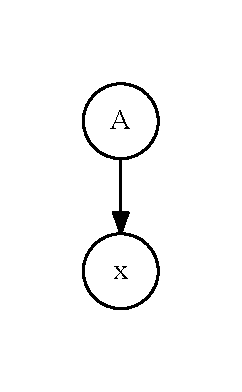
\includegraphics[width=0.2\textwidth]{pictures/tree1.pdf}
 \caption{The derivation tree of the height $h = 1$ for the string $x = l(\pi)$.}
 \label{tree1}
\end{figure}

\textbf{Inductive step}: Assume that the statement of the lemma holds for any $k \leq (p - 1)$ and show that it also holds for $k = p$ where $p \geq 2$. For any $i, j$ and for any non-terminal $A \in N$, $$A \in a^{(p)}_{i,j} \text{ iff } A \in a^{(p-1)}_{i,j} \text{ or } A \in (a^{(p-1)} \times a^{(p-1)})_{i,j},$$ since $$a^{(p)} = a^{(p-1)} \cup (a^{(p-1)} \times a^{(p-1)}).$$

Let $A \in a^{(p-1)}_{i,j}$. By the inductive hypothesis, $A \in a^{(p-1)}_{i,j}$ iff $(i,j) \in R_A$ and there exists $i \pi j$, such that there is a derivation tree of the height $h \leq (p-1)$ for the string $l(\pi)$ and a context-free grammar $G_A = (N,\Sigma,P,A)$. The statement of the lemma holds for $k = p$ since the height $h$ of this tree is also less than or equal to $p$.

Let $A \in (a^{(p-1)} \times a^{(p-1)})_{i,j}$. By the definition of the binary operation $(\cdot)$ on arbitrary subsets, $A \in (a^{(p-1)} \times a^{(p-1)})_{i,j}$ iff there are $r$, $B \in a^{(p-1)}_{i,r}$ and $C \in a^{(p-1)}_{r,j}$, such that $(A \rightarrow B C) \in P$. Hence, by the inductive hypothesis, there are $i \pi_1 r$ and $r \pi_2 j$, such that $(i,r) \in R_B$ and $(r,j) \in R_C$, and there are the derivation trees $T_B$ and $T_C$ of heights $h_1 \leq (p-1)$ and $h_2 \leq (p-1)$ for the strings $w_1 = l(\pi_1)$, $w_2 = l(\pi_2)$ and the context-free grammars $G_B$, $G_C$ respectively. Thus, the concatenation of paths $\pi_1$ and $\pi_2$ is $i \pi j$, where $(i,j) \in R_A$ and there is a derivation tree of the height $h = 1 + max(h_1, h_2)$, shown in Figure~\ref{tree2}, for the string $w = l(\pi)$ and a context-free grammar $G_A$.

\begin{figure}[h!]
 \centering
 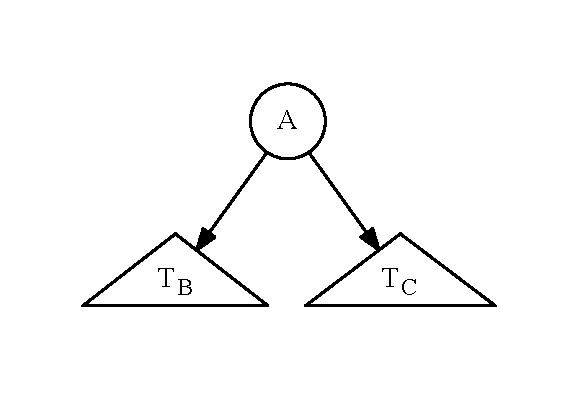
\includegraphics[width=0.8\textwidth]{pictures/tree2.pdf}
 \caption{The derivation tree of the height $h = 1 + max(h_1, h_2)$ for the string $w = l(\pi)$, where $T_B$ and $T_C$ are the derivation trees for strings $w_1$ and $w_2$ respectively.}
 \label{tree2}
\end{figure}

The statement of the lemma holds for $k = p$ since the height $h = 1 + max(h_1, h_2) \leq p$. This completes the proof of the lemma.
\end{proof}

\begin{mytheorem}\label{thm:correct}
 Let $D = (V,E)$ be a graph and let $G =(N,\Sigma,P)$ be a grammar. Then for any $i, j$ and for any non-terminal $A \in N$, $A \in a^{cf}_{i,j}$ iff $(i,j) \in R_A$.
\end{mytheorem}
\begin{proof}

Since the matrix $a^{cf} = a^{(1)} \cup a^{(2)} \cup \cdots,$ for any $i, j$ and for any non-terminal $A \in N$, $A \in a^{cf}_{i,j}$ iff there is $k \geq 1$, such that $A \in a^{(k)}_{i,j}$. By the lemma~\ref{lemma:cf}, $A \in a^{(k)}_{i,j}$ iff $(i,j) \in R_A$ and there is $i \pi j$, such that there is a derivation tree of the height $h \leq k$ for the string $l(\pi)$ and a context-free grammar $G_A = (N,\Sigma,P,A)$. This completes the proof of the theorem.
\end{proof}

We can, therefore, determine whether $(i,j) \in R_A$ by asking whether $A \in a^{cf}_{i,j}$. Thus, we show how the context-free relations $R_A$ can be calculated by computing the transitive closure $a^{cf}$ of the matrix $a$.



\subsection{The algorithm} \label{section_algorithm}
In this section, we introduce an algorithm for calculating the transitive closure $a^{cf}$ which was discussed in Section~\ref{section_reducing}.

Let $D = (V, E)$ be the input graph and $G = (N,\Sigma,P)$ be the input grammar.

\begin{algorithm}[H]
\begin{algorithmic}[1]
\caption{Context-free recognizer for graphs}
\label{alg:graphParse}
\Function{contextFreePathQuerying}{D, G}
    
    \State{$n \gets$ the number of nodes in $D$}
    \State{$E \gets$ the directed edge-relation from $D$}
    \State{$P \gets$ the set of production rules in $G$}
    \State{$T \gets$ the matrix $n \times n$ in which each element is $\varnothing$}
    \ForAll{$(i,x,j) \in E$}
    \Comment{Matrix initialization}
        \State{$T_{i,j} \gets T_{i,j} \cup \{A~|~(A \rightarrow x) \in P \}$}
    \EndFor    
    \While{matrix $T$ is changing}
       
        \State{$T \gets T \cup (T \times T)$}
        \Comment{Transitive closure $T^{cf}$ calculation} 
    \EndWhile
\State \Return $T$
\EndFunction
\end{algorithmic}
\end{algorithm}

Note that the matrix initialization in lines \textbf{6-7} of the Algorithm~\ref{alg:graphParse} can handle arbitrary graph $D$. For example, if a graph $D$ contains multiple edges $(i,x_1,j)$ and $(i,x_2,j)$ then both the elements of the set $\{A~|~(A \rightarrow x_1) \in P \}$ and the elements of the set $\{A~|~(A \rightarrow x_2) \in P \}$ will be added to $T_{i,j}$.

We need to show that the Algorithm~\ref{alg:graphParse} terminates in a finite number of steps. Since each element of the matrix $T$ contains no more than $|N|$ non-terminals, the total number of non-terminals in the matrix $T$ does not exceed $|V|^2|N|$. Therefore, the following theorem holds.

\begin{mytheorem}\label{thm:finite}
 Let $D = (V,E)$ be a graph and let $G =(N,\Sigma,P)$ be a grammar. The Algorithm~\ref{alg:graphParse} terminates in a finite number of steps. 
\end{mytheorem}
\begin{proof}
It is sufficient to show, that the operation in the line \textbf{9} of the Algorithm~\ref{alg:graphParse} changes the matrix $T$ only finite number of times. Since this operation can only add non-terminals to some elements of the matrix $T$, but not remove them, it can change the matrix $T$ no more than $|V|^2|N|$ times.
\end{proof}

Denote the number of elementary operations executed by the algorithm of multiplying two $n \times n$ Boolean matrices as $BMM(n)$. According to Valiant, the matrix multiplication operation in the line \textbf{9} of the Algorithm~\ref{alg:graphParse} can be calculated in $O(|N|^2 BMM(|V|))$. Denote the number of elementary operations executed by the matrix union operation of two $n \times n$ Boolean matrices as $BMU(n)$. Similarly, it can be shown that the matrix union operation in the line \textbf{9} of the Algorithm~\ref{alg:graphParse} can be calculated in $O(|N|^2 BMU(n))$. Since the line \textbf{9} of the Algorithm~\ref{alg:graphParse} is executed no more than $|V|^2|N|$ times, the following theorem holds.

\begin{mytheorem}\label{thm:time}
 Let $D = (V,E)$ be a graph and let $G =(N,\Sigma,P)$ be a grammar. The Algorithm~\ref{alg:graphParse} calculates the transitive closure $T^{cf}$ in $O(|V|^2|N|^3(BMM(|V|) + BMU(|V|)))$.
\end{mytheorem}

We also provide the worst-case example, for which the time complexity in terms of the graph size provided by Theorem~\ref{thm:time} cannot be improved. This example is based on the context-free grammar $G = (N, \Sigma, P)$ where:
\begin{itemize}
	\item the set of non-terminals $N = \{S\}$;
	\item the set of terminals $\Sigma = \{a, b\}$;
	\item the set of production rules $P$ is presented on Figure~\ref{ProductionRulesWorsCaseExample}.
\end{itemize}

\begin{figure}[h]
	\[
	\begin{array}{rccl}
	0: & S & \rightarrow & \text{\emph{a}} \ S \ \text{\emph{b}} \\
	1: & S & \rightarrow & \text{\emph{a}} \ \text{\emph{b}} \\ 
	\end{array}
	\]
	\caption{Production rules for the worst-case example.}
	\label{ProductionRulesWorsCaseExample}
\end{figure}

Let the size $|N|$ of the grammar $G$ be a constant. The worst-case time complexity is reached by running this query on the double-cyclic graph where:
\begin{itemize}
	\item one of the cycles having $u = 2^k + 1$ edges labeled with $a$;
	\item another cycle having $v = 2^k$ edges labeled with $b$;
	\item the two cycles are connected via a shared node $m$.
\end{itemize}

A small example of such graph with $k = 1$, $u = 3$, $v = 2$, and $m = 0$ is presented on Figure~\ref{worst_case_graph}.

\begin{figure}[h]
	\[
	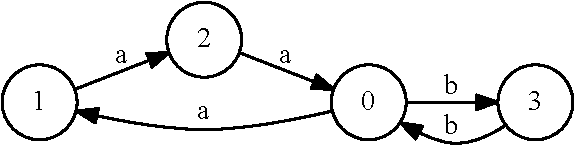
\includegraphics[width=0.8\textwidth]{pictures/worst_case_graph.pdf}
	\]
	\caption{An example of the graph for the worst-case time complexity.}
	\label{worst_case_graph}
\end{figure}

The shortest path $\pi$ from the node $m$ to the node $m$, whose labeling forms a string from the language $L(G_S)=\{a^n b^n; n \geq 1\}$, has a length $l = 2*u*v$, since $u = 2^k + 1$ and $v = 2^k$ are coprime, and string $s$, formed by this path, consists of $u*v$ labels $a$ and $u*v$ labels $b$. The string $s = l(\pi)$ has a derivation tree according to a context-free grammar $G_S$ of the minimal height $h = 2*u*v$ among all the paths from the node $m$ to the node $m$ in this double-cyclic graph. Therefore, if we run the worst-case example query on this graph, then the operation in the line \textbf{9} of the Algorithm~\ref{alg:graphParse} changes the matrix $T$ at least $h = 2*u*v$ times. Hence, the Algorithm~\ref{alg:graphParse} computes this query in $O(|V|^2(BMM(|V|) + BMU(|V|)))$, since $|V| = (u + v - 1) = 2*v$ and $h = 2*u*v > 2*v*v = |V|^2 / 4 = O(|V|^2)$.


\subsection{An example} \label{section_example}
In this section, we provide a step-by-step demonstration of the proposed algorithm. For this, we consider the classical \textit{same-generation query}~\cite{FndDB}.

The \textbf{example query} is based on the context-free grammar $G = (N, \Sigma, P)$ where:
\begin{itemize}
    \item The set of non-terminals $N = \{S\}$.
    \item The set of terminals $$\Sigma = \{subClassOf, subClassOf^{-1}, type, type^{-1}\}.$$
    \item The set of production rules $P$ is presented in Figure~\ref{ProductionRulesExampleQuery}.
\end{itemize}

\begin{figure}[h]
   \[
\begin{array}{rccl}
   0: & S & \rightarrow & \text{\textit{subClassOf}}^{-1} \ S \ \text{\textit{subClassOf}} \\ 
   1: & S & \rightarrow & \text{\textit{type}}^{-1} \ S \ \text{\textit{type}} \\ 
   2: & S & \rightarrow & \text{\textit{subClassOf}}^{-1} \ \text{\textit{subClassOf}} \\ 
   3: & S & \rightarrow & \text{\textit{type}}^{-1} \ \text{\textit{type}} \\ 
\end{array}
\]
\caption{Production rules for the example query grammar.}
\label{ProductionRulesExampleQuery}
\end{figure}

Since the proposed algorithm processes only grammars in Chomsky normal form, we first transform the grammar $G$ into an equivalent grammar $G' = (N', \Sigma', P')$ in normal form, where:
\begin{itemize}
    \item The set of non-terminals $N' = \{S, S_1, S_2, S_3, S_4, S_5, S_6\}$.
    \item The set of terminals $$\Sigma' = \{subClassOf, subClassOf^{-1}, type, type^{-1}\}.$$
    \item The set of production rules $P'$ is presented in Figure~\ref{ProductionRulesExampleQueryCNF}.
\end{itemize}

\begin{figure}[h]
   \[
\begin{array}{rccl}
   0: & S & \rightarrow & S_1 \ S_5 \\
   1: & S & \rightarrow & S_3 \ S_6 \\
   2: & S & \rightarrow & S_1 \ S_2 \\
   3: & S & \rightarrow & S_3 \ S_4 \\
   4: & S_5 & \rightarrow & S \ S_2 \\
   5: & S_6 & \rightarrow & S \ S_4 \\
   6: & S_1 & \rightarrow & \text{\textit{subClassOf}}^{-1} \\ 
   7: & S_2 & \rightarrow & \text{\textit{subClassOf}} \\ 
   8: & S_3 & \rightarrow & \text{\textit{type}}^{-1} \\
   9: & S_4 & \rightarrow & \text{\textit{type}} \\ 
\end{array}
\]
\caption{Production rules for the example query grammar in normal form.}
\label{ProductionRulesExampleQueryCNF}
\end{figure}

We run the query on a graph presented in Figure~\ref{ExampleQueryGraph}.

\begin{figure}[h]
\[
    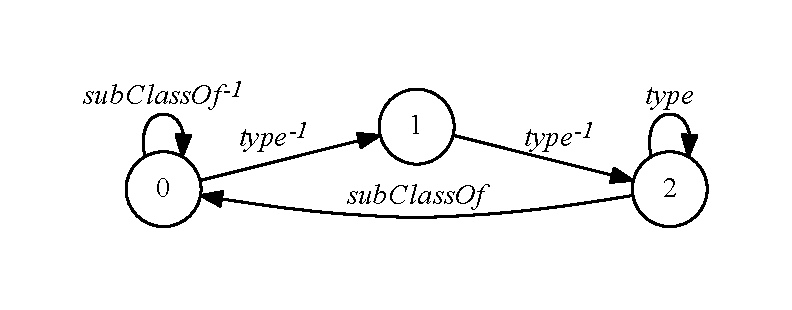
\includegraphics[width=0.8\textwidth]{pictures/ExampleGraph.pdf}
\]
\caption{An input graph for the example query.}
\label{ExampleQueryGraph}
\end{figure}

We provide a step-by-step demonstration of the work with the given graph $D$ and grammar $G'$ of the Algorithm~\ref{alg:graphParse}. After the matrix initialization in lines \textbf{6-7} of the Algorithm~\ref{alg:graphParse}, we have a matrix $T_0$ presented in Figure~\ref{ExampleQueryInitMatrix}.

\begin{figure}[h]
\[
T_0 = \begin{pmatrix}
    \{S_1\} & \{S_3\} & \varnothing \\ \varnothing & \varnothing & \{S_3\} \\ \{S_2\} & \varnothing & \{S_4\}
\end{pmatrix}
\]
\caption{The initial matrix for the example query.}
\label{ExampleQueryInitMatrix}
\end{figure}

Let $T_i$ be the matrix $T$ obtained after executing the loop in lines \textbf{8-9} of the Algorithm~\ref{alg:graphParse} $i$ times. The calculation of the matrix $T_1$ is shown in Figure~\ref{ExampleQueryFirstIteration}.

\begin{figure}[h]
\[
T_0 \times T_0 = \begin{pmatrix}
    \varnothing & \varnothing & \varnothing \\ \varnothing & \varnothing & \{S\} \\ \varnothing & \varnothing & \varnothing
\end{pmatrix}
\]

\[
T_1 = T_0 \cup (T_0 \times T_0) = \begin{pmatrix}
    \{S_1\} & \{S_3\} & \varnothing \\ \varnothing & \varnothing & \{S_3, S\} \\ \{S_2\} & \varnothing & \{S_4\}
\end{pmatrix}
\]
\caption{The first iteration of computing the transitive closure for the example query.}
\label{ExampleQueryFirstIteration}
\end{figure}

When the algorithm at some iteration finds new paths in the graph $D$, then it adds corresponding nonterminals to the matrix $T$. For example, after the first loop iteration, non-terminal $S$ is added to the matrix $T$. This non-terminal is added to the element with a row index $i = 1$ and a column index $j = 2$. This means that there is $i\pi j$ (a path $\pi$ from the node 1 to the node 2), such that $S \xrightarrow{*} l(\pi)$. For example, such a path consists of two edges with labels $type^{-1}$ and $type$, and thus $S \xrightarrow{*} type^{-1} \ type$.

The calculation of the transitive closure is completed after $k$ iterations when a fixpoint is reached: $T_{k-1} = T_k$. For the example query, $k = 6$ since $T_6 = T_5$. The remaining iterations of computing the transitive closure are presented in Figure~\ref{ExampleQueryFinalIterations}.

\begin{figure}[h]
\[
T_2 = \begin{pmatrix}
    \{S_1\} & \{S_3\} & \varnothing \\ \{S_5\} & \varnothing & \{S_3, S, S_6\} \\ \{S_2\} & \varnothing & \{S_4\}
\end{pmatrix}
\]

\[
T_3 = \begin{pmatrix}
    \{S_1\} & \{S_3\} & \{S\} \\ \{S_5\} & \varnothing & \{S_3, S, S_6\} \\ \{S_2\} & \varnothing & \{S_4\}
\end{pmatrix}
\]

\[
T_4 = \begin{pmatrix}
    \{S_1, S_5\} & \{S_3\} & \{S, S_6\} \\ \{S_5\} & \varnothing & \{S_3, S, S_6\} \\ \{S_2\} & \varnothing & \{S_4\}
\end{pmatrix}
\]

\[
T_5 = \begin{pmatrix}
    \{S_1, S_5, S\} & \{S_3\} & \{S, S_6\} \\ \{S_5\} & \varnothing & \{S_3, S, S_6\} \\ \{S_2\} & \varnothing & \{S_4\}
\end{pmatrix}
\]
\caption{Remaining states of the matrix $T$.}
\label{ExampleQueryFinalIterations}
\end{figure}

Thus, the result of the Algorithm~\ref{alg:graphParse} for the example query is the matrix $T_5 = T_6$. Now, after constructing the transitive closure, we can construct the context-free relations $R_A$. These relations for each non-terminal of the grammar $G'$ are presented in Figure~\ref{ExampleQueryCFRelations}.

\begin{figure}[h]
\begin{eqnarray*}
R_S&=&\{(0,0),(0,2),(1,2)\},\\
R_{S_1}&=&\{(0,0)\},\\
R_{S_2}&=&\{(2,0)\}, \\
R_{S_3}&=&\{(0,1), (1,2)\}, \\
R_{S_4}&=&\{(2,2)\}, \\
R_{S_5}&=&\{(0,0), (1,0)\}, \\
R_{S_6}&=&\{(0,2), (1,2)\}.
\end{eqnarray*}
\caption{Context-free relations for the example query.}
\label{ExampleQueryCFRelations}
\end{figure}

By the context-free relation $R_S$, we can conclude that there are paths in a graph $D$ only from the node 0 to the node 0, from the node 0 to the node 2 or from the node 1 to the node 2, corresponding to the context-free grammar $G_S$. This conclusion is based on the fact that a grammar $G'_S$ is equivalent to the grammar $G_S$ and $L(G_S) = L(G_S')$.

\section{Доказательство корректности алгоритма}
\textsc{Свойство 1.} 
\textit{Алгоритм завершает работу для любых входных данных.}

\textsc{Доказательство.}
С каждой вершиной внутреннего представления графа входного конечного автомата ассоциировано не более $N$ вершин графа GSS, где $N$~--- количество состояний синтаксического анализатора. Таким образом, количество вершин в графе GSS ограничено сверху числом $N \times n$, где $n$~--- количество вершин графа входного автомата. Так как в GSS нет кратных рёбер, количество его рёбер~--- $O((N \times n)^{2})$. На каждой итерации основного цикла алгоритм извлекает из очереди $Q$ и обрабатывает одну вершину внутреннего графа. Вершины добавляются в очередь $Q$, только когда происходит добавление нового ребра в GSS. Так как количество рёбер в GSS конечно, алгоритм завершает работу для любых входных данных. $\square$~\\~

Для того, чтобы доказать корректность построения конечного представления леса 
разбора, нам потребуется следующее определение.~\\~

\textsc{Определение 1.} 
\emph{Корректное дерево}~--- это упорядоченное дерево со следующими свойствами.
\begin{enumerate}
  \item Корень дерева соответствует стартовому нетерминалу грамматики $G$.
  \item Листья соответствуют терминалам грамматики $G$. Упорядоченная последовательность листьев соответствует некоторому пути во входном графе.
  \item Внутренние узлы соответствуют нетерминалам грамматики $G$. Дети внутреннего узла (для нетерминала $N$) соответствуют символам правой части некоторой продукции для $N$ в грамматике $G$.
\end{enumerate}

Неформально корректное дерево~--- это дерево вывода некоторой цепочки из 
регулярного множества в эталонной грамматике. Далее нам необходимо доказать, 
во-первых, что конечное представление леса разбора SPPF содержит только 
корректные деревья, и во-вторых, что для каждой корректной относительно 
эталонной грамматики цепочки существует корректное дерево вывода в SPPF.~\\~

\textsc{Лемма.}
\textit{Для каждого ребра GSS $(v_{t}, v_{h})$ такого, что $v_{t} \in V_{t}.processed$, $v_{h} \in V_{h}.processed$, терминалы ассоциированного поддерева соответствуют некоторому пути во входном графе из вершины $V_{h}$ в $V_{t}$.}

\textsc{Доказательство.}
Будем строить доказательство при помощи индукции по высоте дерева вывода. База: либо 
$\epsilon$-дерево, либо дерево, состоящее из единственной вершины-терминала. 
$\epsilon$-дерево соответствует пути длины $0$; начальная и конечная вершины 
ребра, соответствующего такому дереву, совпадают, поэтому утверждение верно. 
Дерево, состоящее из одной вершины, соответствует терминалу, считанному с 
некоторого ребра $(V_{h}, V_{t})$ внутреннего графа, поэтому утверждение верно.

Корнем дерева высоты $k$ является некий нетерминал $N$. По третьему пункту 
определения корректного дерева существует некоторое правило эталонной 
грамматики $N \rightarrow A_{0}, A_{1}, \dots, A_{n}$, где $A_{0}, A_{1}, 
\dots, A_{n}$ являются детьми корневого узла. Поддерево $A_{i}$ 
ассоциировано с ребром $(v_{t}^{i}, v_{h}^{i})$ графа GSS и, так как его 
высота равна $k-1$, то по индукционному предположению существует путь во 
внутреннем графе из вершины $V_{h}^{i}$ в вершину $V_{t}^{i}$. Вершина 
$V_{t}^{i} = V_{h}^{i+1}$, так как $v_{t}^{i} = v_{h}^{i+1}$, поэтому во 
внутреннем графе существует путь из вершины $V_{h}^{0}$ в вершину 
$V_{t}^{n}$, соответствующий рассматриваемому корректному дереву. $\square$~\\~

\textsc{Свойство 2.} 
\textit{Любое дерево, сгенерированное из SPPF, является корректным.}

\textsc{Доказательство.}
Рассмотрим произвольное сгенерированное из SPPF дерево и докажем, что оно 
удовлетворяет определению 1. Первый и третий пункт определения корректного дерева следует из определения SPPF. Второй пункт определения следует из \textsc{леммы}, если применить её к рёбрам GSS, начало которых лежит на последнем уровне стека и помечено принимающим состоянием, а конец~--- в вершинах на уровне 0. $\square$~\\~

\textsc{Свойство 3.} 
\textit{Для каждой корректной относительно эталонной грамматики строки, соответствующей пути $p$ во входном графе, из SPPF может быть порождено корректное дерево, соответствующее пути $p$.}

\textsc{Доказательство.}
Рассмотрим произвольное корректное дерево и докажем, что оно может быть порождено из SPPF. Доказательство повторяет доказательство корректности для RNGLR-алгоритма, за исключением следующего момента. RNGLR-алгоритм строит граф GSS по слоям: гарантируется, что $\forall j \in [0..i-1], j-$ый уровень GSS будет зафиксирован на момент построения $i-$ого уровня. В нашем случае это свойство не верно, что может приводить к возможному порождению новых путей для свёрток, которые были ранее обработаны. Единственный возможный способ добавления такого нового пути~--- это добавление ребра $(v_{t}, v_{h})$, где вершина $v_{t}$ ранее присутствовала в GSS и имела входящие ребра. Так как алгоритм сохраняет информацию о том, какие свёртки проходили через вершины GSS, достаточно продолжить свёртки, проходящие через вершину $v_{t}$, и это ровно то, что делает функция \emph{applyPassingReductions}. $\square$~\\~

\textsc{Замечание.} Построение леса разбора осуществляется одновременно с построением GSS, при этом дерево вывода нетерминала ассоциируется с ребром GSS каждый раз при обработке соответствующей свёртки, вне зависимости от того, было ли ребро в графе до этого, либо добавлено на данном шаге. Это обстоятельство позволяет утверждать, что если все возможные редукции были выполнены, то и лес разбора содержит все деревья для всех корректных цепочек из аппроксимации.

\section{Экспериментальное исследование}
Предложенный механизм диагностики ошибок был реализован на платформе .NET как часть проекта YaccConstructor; основным языком разработки являлся F\#~\cite{FSharp}. Данная реализация является модификацией ранее реализованного в рамках проекта алгоритма ослабленного синтаксического анализа регулярной аппроксимации динамически формируемого выражения.

Модифицированный алгоритм был протестирован на серии тестов с целью проверки работоспособности. Данные тесты проверяли, что алгоритм строит корректные множества $errors$ и $probErrors$ ребер входного графа. Для каждого теста специфицировалась грамматика на языке YARD и в явном виде задавался граф конечного автомата, ребра которого были промаркированы лексемами входной грамматики. Входные графы для данных тестов содержали как ветвления, так и циклы. На всех тестах модифицированный алгоритм корректно строил множества $errors$ и $probErrors$. Кроме того, на всех тестах, входные графы которых не содержали циклов, модифицированный алгоритм точно определял все ошибочные ребра входного графа, то есть $probErrors$, в данном случае, являлось пустым множеством.

Также на нескольких сериях синтетических тестов была протестирована производительность модифицированного алгоритма. Анализ промышленного проекта по миграции базы данных с MS-SQL Server 2005 на Oracle 11gR2 показал, что запросы часто формируются конкатенацией фрагментов, каждый из которых формируется с помощью ветвлений или циклов. Ниже приведена входная грамматика, использованная в данных тестах:
$$
\begin{array}{crcl}
& start\_rule &::=& s \\
& s & ::= & s \mbox{\texttt{ PLUS }} \mbox{\texttt{n}}\\
& n & ::= & \mbox{\texttt{ONE | }} \mbox{\texttt{TWO | }} \mbox{\texttt{THREE | }} \mbox{\texttt{FIVE | }} \mbox{\texttt{SIX | }} \mbox{\texttt{SEVEN}}
\end{array}
$$
Входные графы представляли собой конкатенацию базовых блоков без циклов. Каждая серия тестов характеризовалась тремя параметрами: 
\begin{itemize}
  \item $height$~--- количество ветвлений в базовом блоке;
  \item $length$~--- максимальное количество повторений базовых блоков;
  \item $errorBranches$~--- количество веток в базовом блоке, содержащих ошибочное ребро (на рис.~\ref{block} изображен базовый блок без ошибочных ребер, а на рис.~\ref{errorBlock} --- базовый блок с двумя выделенными ошибочными ребрами).
\end{itemize}

\begin{figure}[h!]
 \centering
 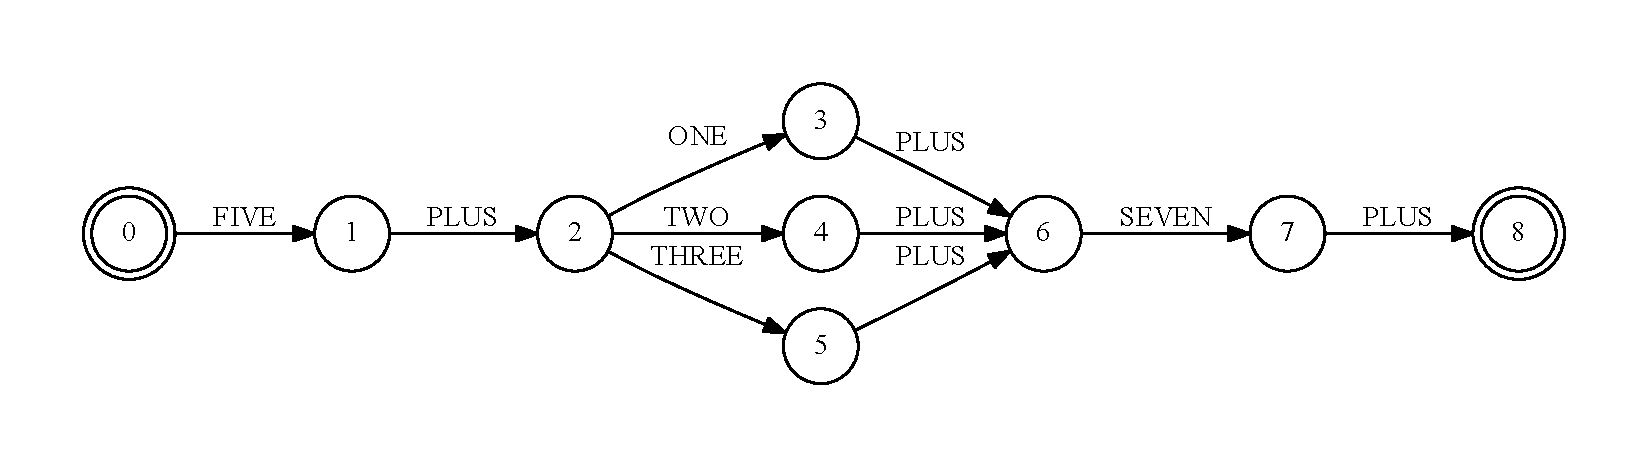
\includegraphics[width=\textwidth]{Azimov/pictures/block_black.pdf}
 \caption{Базовый блок при $height=3, errorBranches=0$}
 \label{block}
\end{figure}

\begin{figure}[h!]
 \centering
 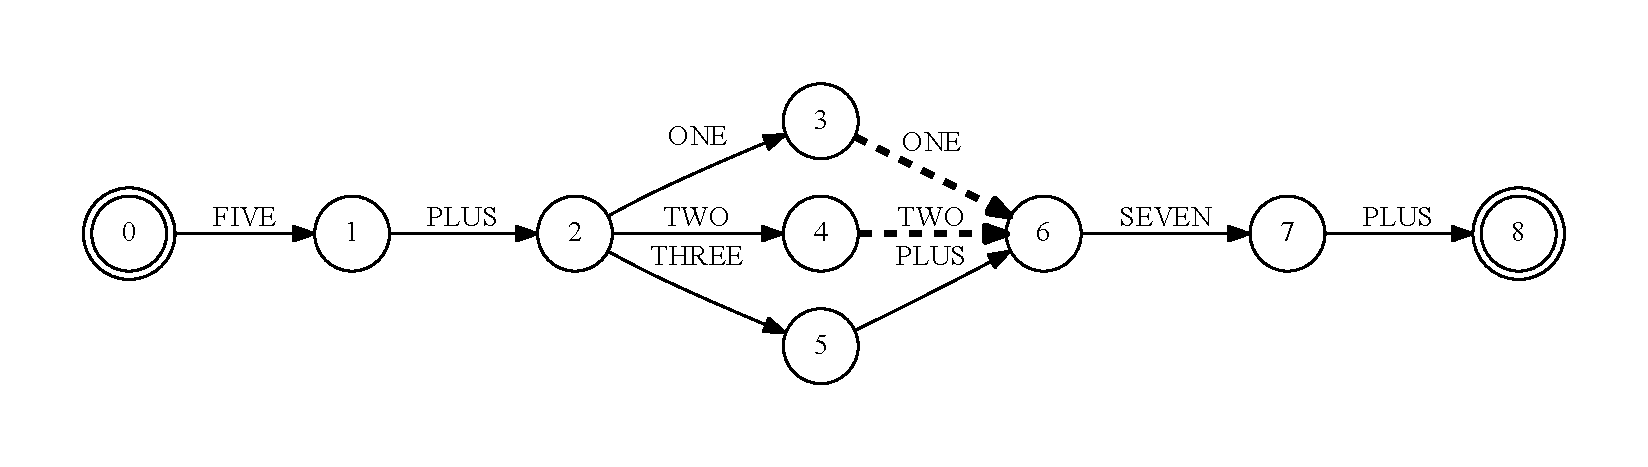
\includegraphics[width=\textwidth]{Azimov/pictures/errorBlock_black.pdf}
 \caption{Базовый блок при $height=3, errorBranches=2$}
 \label{errorBlock}
\end{figure}

Замеры времени работы алгоритмов проводились на машине со следующими техническими характеристиками: Intel(R) Core(TM) i7-3630QM CPU @ 2.40GHz, RAM: 8.0~GB, процессор x64.

\begin{figure}[H]
 \centering
 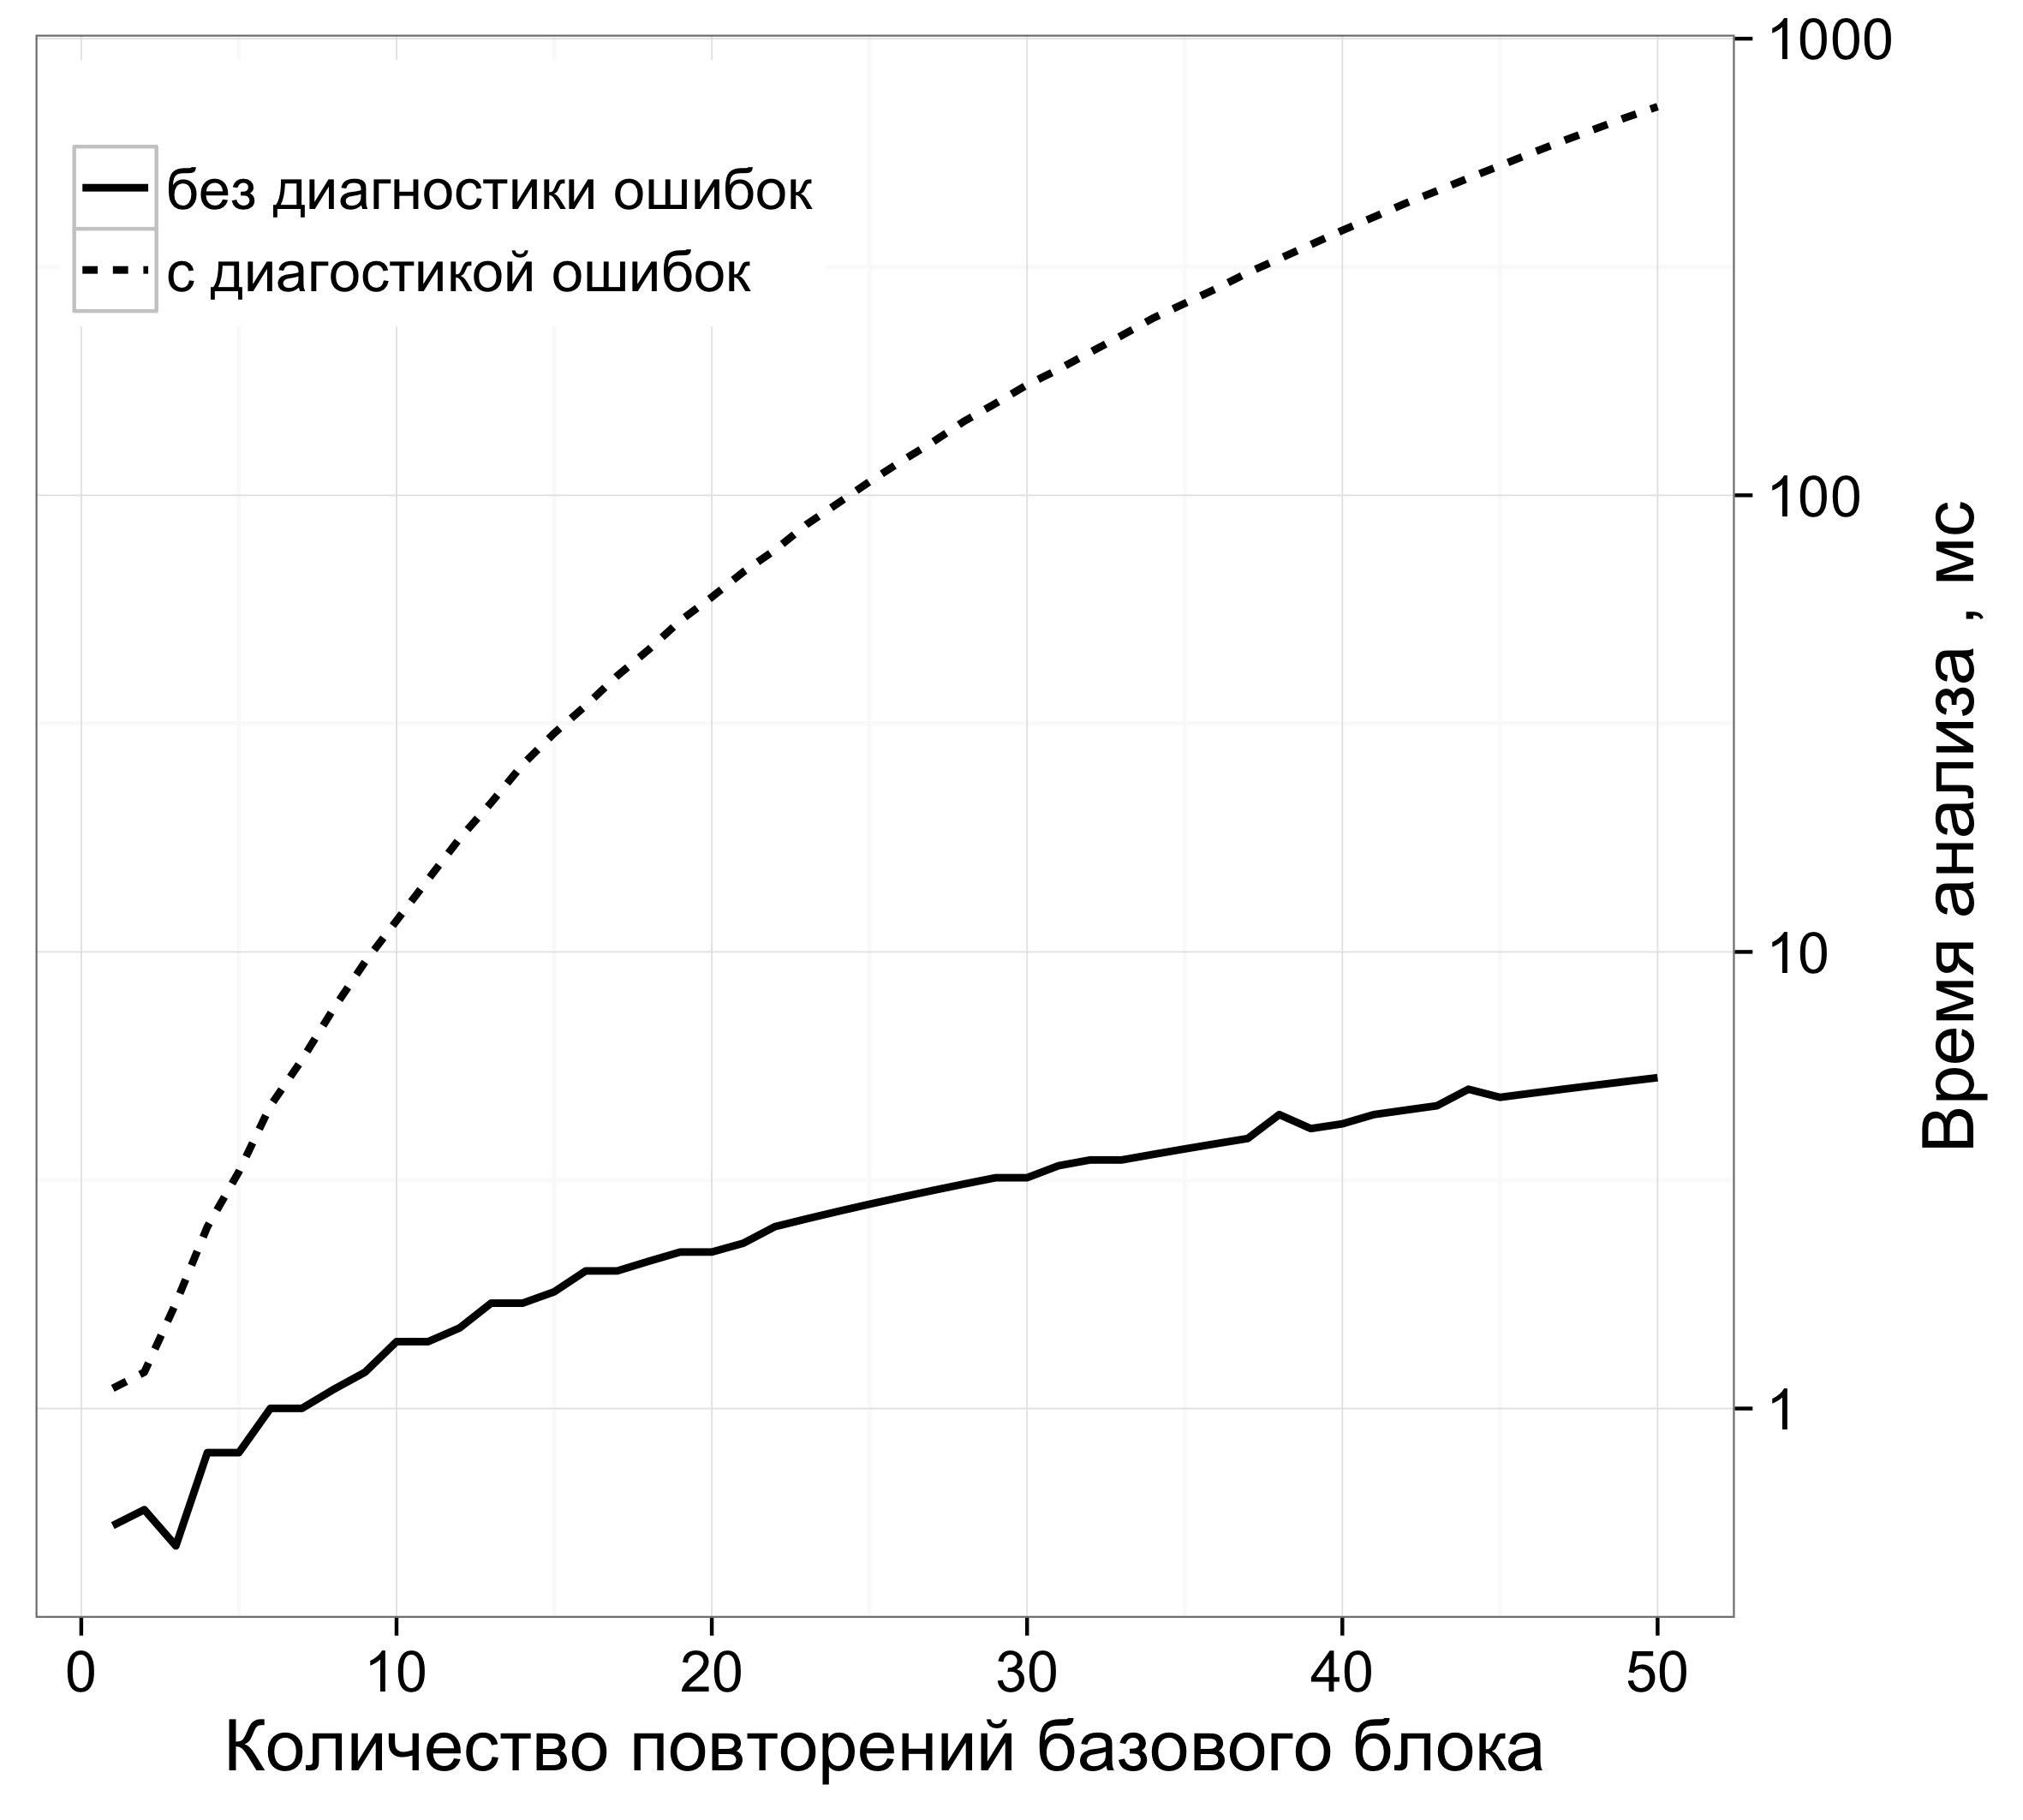
\includegraphics[width=0.9\textwidth]{Azimov/pictures/compare_black.png}
 \caption{Сравнение времени работы алгоритма синтаксического анализа до и после модификаций, при $height=4, errors=0$}
 \label{compare}
\end{figure}


Каждая серия объединяет набор из 50 тестов, каждый из которых содержит одинаковое количество ветвлений в базовом блоке, при этом количество повторений блока совпадает с порядковым номером теста ($length = i$, для теста с номером $i$). Для каждого теста измерялось время, затраченное на синтаксический анализ. Измерения проводились 10 раз, после чего усреднялись. График, представленный на рис.~\ref{compare}, иллюстрирует сравнение времени работы алгоритма синтаксического анализа до и после модификаций. Можно заметить, что выполненная модификация существенно увеличивает продолжительность анализа. Причина этого в том, что выполненная модификация является прототипом, а в будущем планируется улучшить производительность путем улучшения реализации. График на рис.~\ref{withErrors} демонстрирует зависимость времени работы модифицированного алгоритма от количества повторений базового блока и количества веток, содержащих ошибочное ребро, в каждом из них. Наблюдается уменьшение времени работы модифицированного алгоритма при увеличении количества ошибочных ребер. Одной из причин этого является уменьшение количества корректных префиксов внутреннего графа при увеличении количества ошибочных ребер.

\begin{figure}[H]
 \centering
 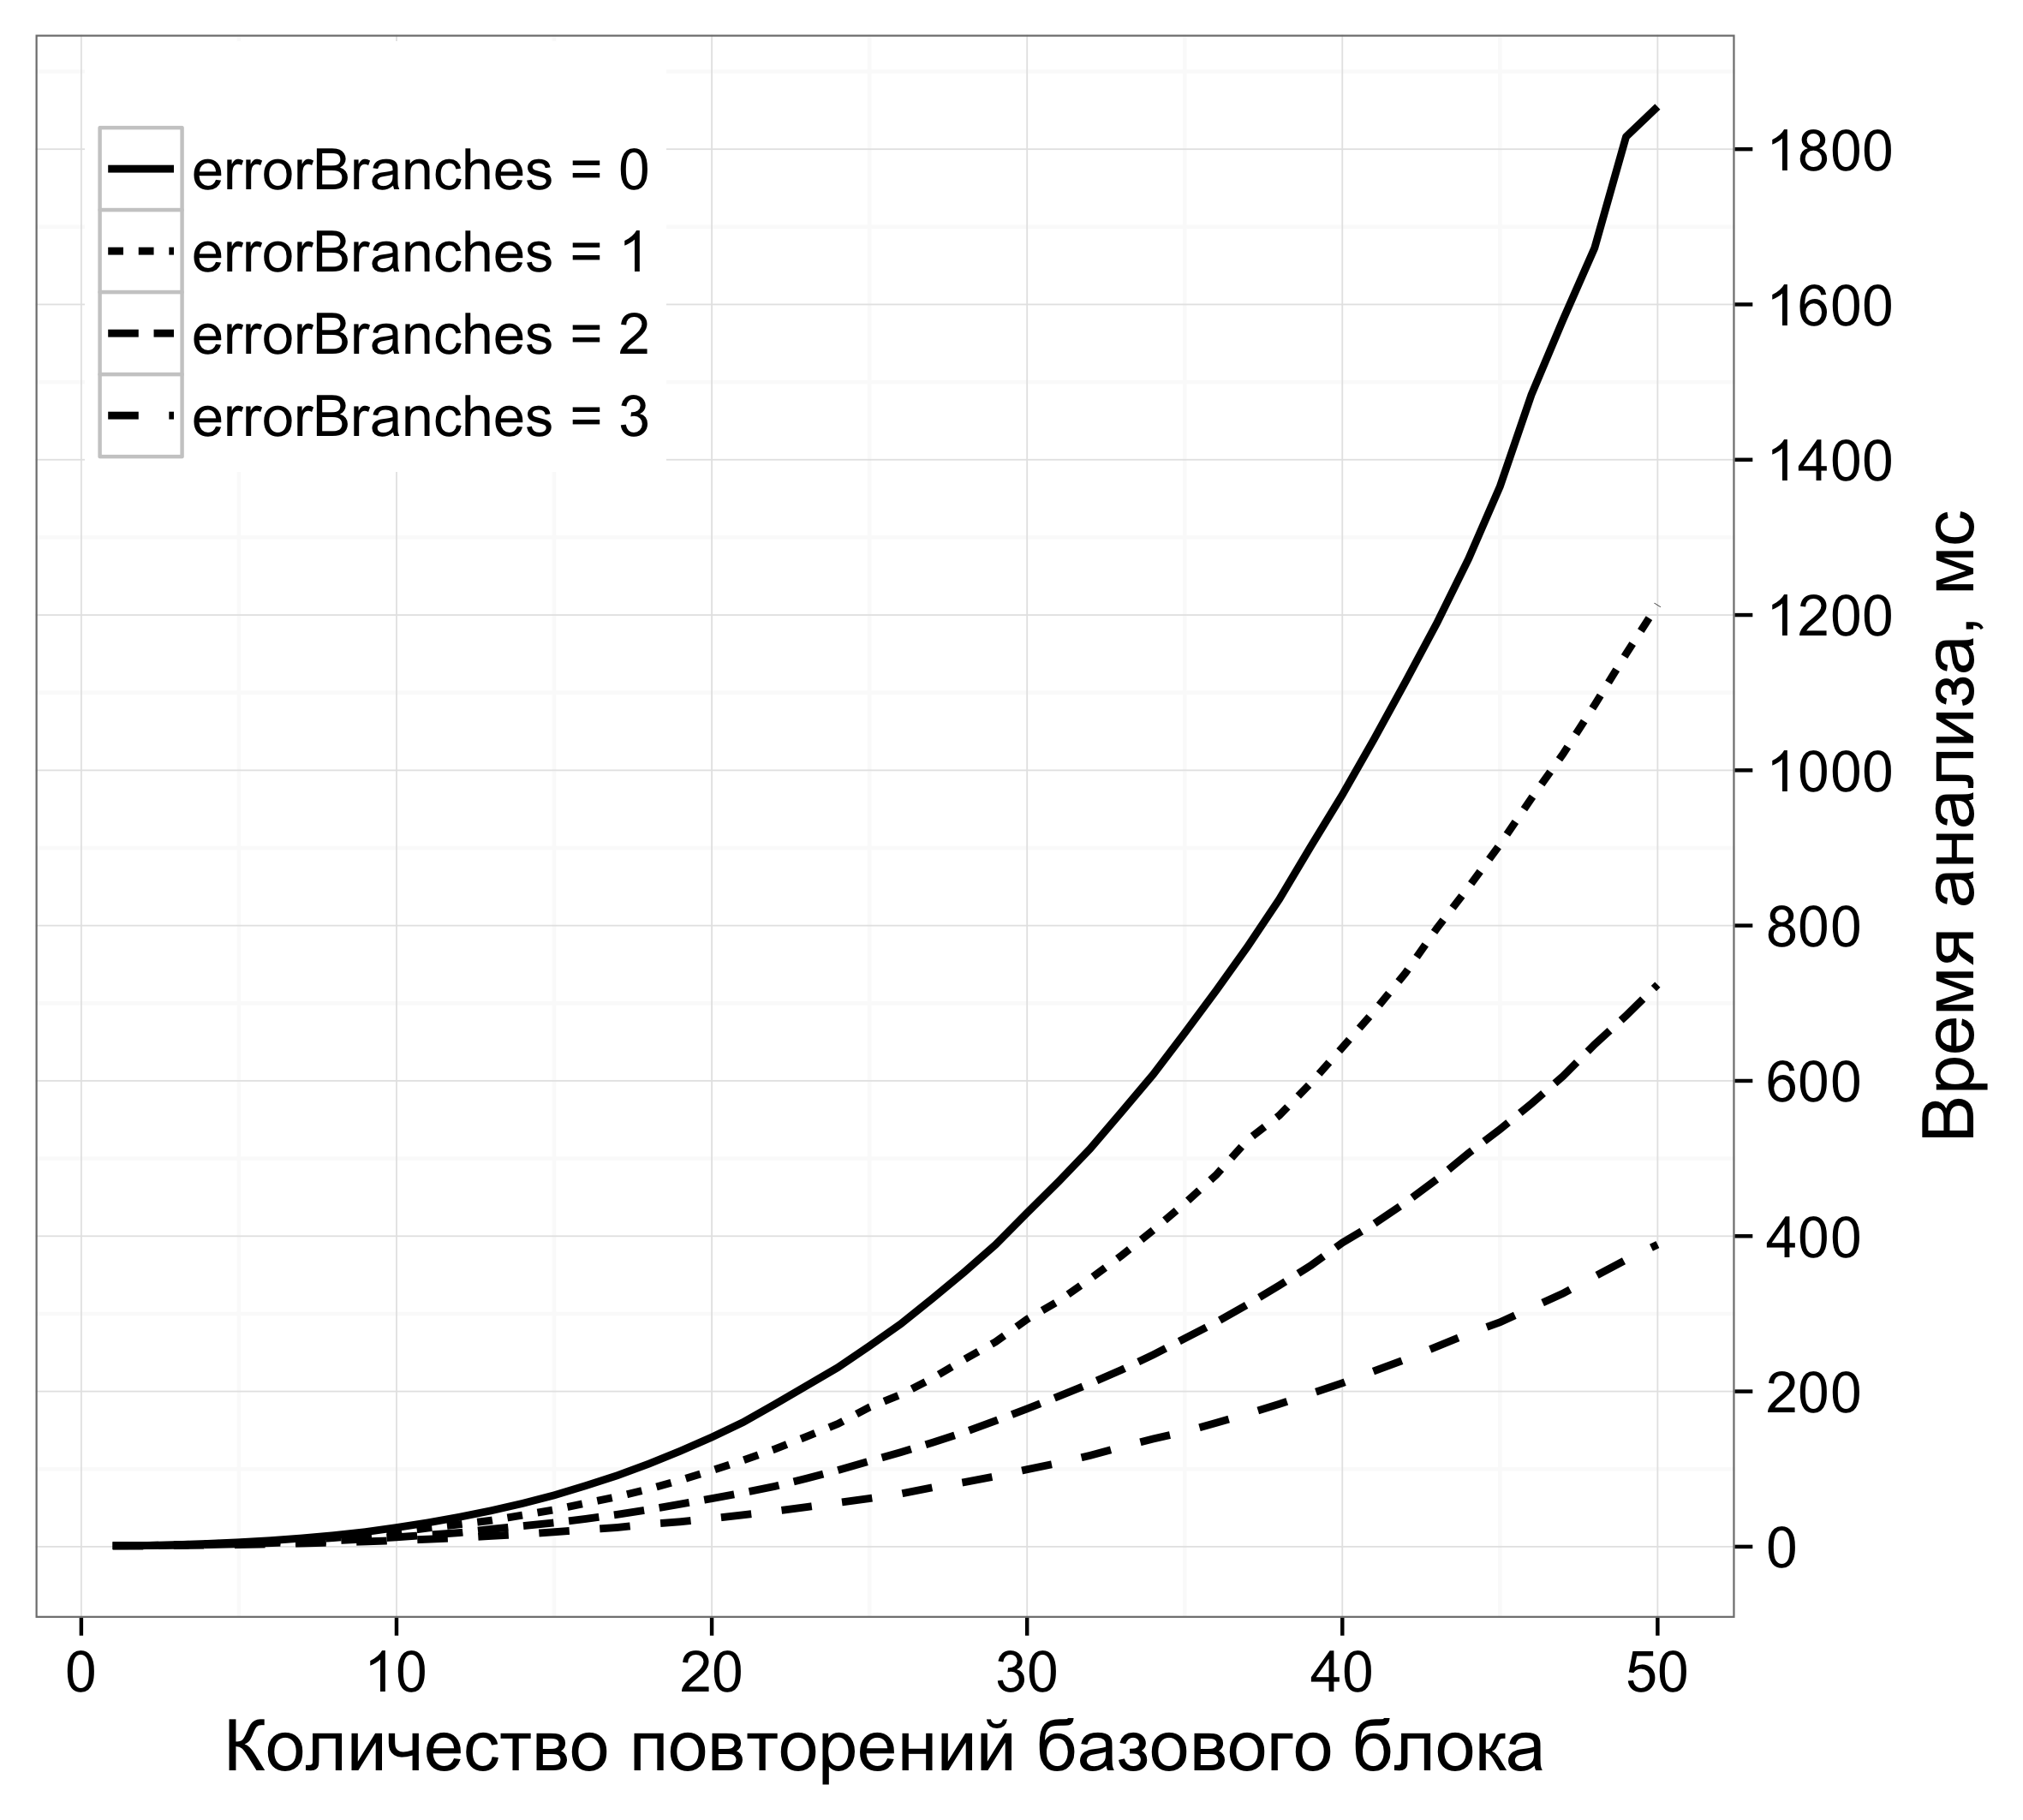
\includegraphics[width=0.9\textwidth]{Azimov/pictures/error_branches4_black.png}
 \caption{Зависимость времени работы модифицированного алгоритма от размера входного графа и количества ошибочных ребер при $height=6$}
 \label{withErrors}
\end{figure}

\section{Заключение}

В данной работе описан подход к композициональному символьному исполнению без раскрутки. Была предложена концепция композициональной памяти с символьной адресацией. Был доказан некоторый набор свойств КСП, дающий основание для подхода в стиле систем переписывания, где символьные кучи могут сами выступать как символы. Это даёт возможность автоматически порождать уравнения на состояния, решения которых в точности отражают поведения функций, работающих с динамической памятью. Было показано как свести задачу решения уравнений на состояния к задаче проверки безопасности чистых функций второго порядка.

Данная работа нацелена на теоретические основания композиционального анализа динамической памяти. Мы оставляем апробацию этого подхода на будущее. Другим направлением будущих исследований может быть расширение нашего формализма на композициональный анализ параллельных программ.

\bibliographystyle{ugost2008ls}
\bibliography{diploma.bib}
\end{document}
